\section{Solution}

%----------------------------------------------------------------------------------------
%	PROJECT STRUCTURE SUBSECTION
%----------------------------------------------------------------------------------------
\subsection{Project Structure}
Project contains 2 folders Core and Drivers. In Core folder I implemented a basic structure that describes a connection to micro-controller and implemented basic function as read write connect. In the second folder Drivers I added drivers for LCD.\\\\
\centerline{
	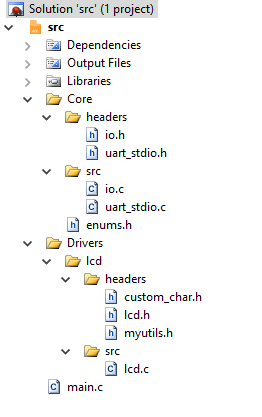
\includegraphics[width=0.5\textwidth]{solution/images/src.png}
}

%----------------------------------------------------------------------------------------
%	PROTEUS SUBSECTION
%----------------------------------------------------------------------------------------

\newpage
\subsection{Circuit in Proteus}
This is circuit in Proteus that is composed from a LCD a led and a button\\\\
\centerline{
	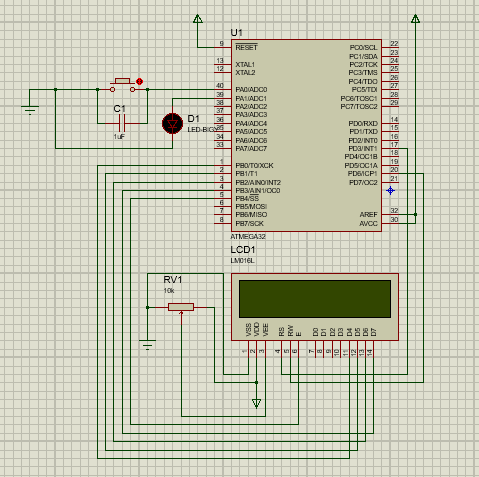
\includegraphics[width=1.0\textwidth]{solution/images/schematics1.png}
}

\newpage
\subsubsection{Let's take a look close at LCD connection \\}
\centerline{
	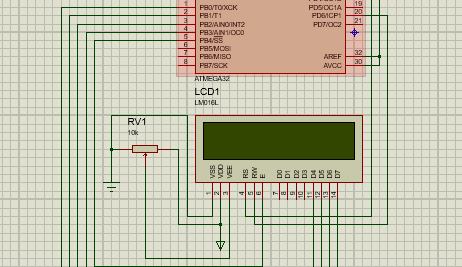
\includegraphics[width=0.7\textwidth]{solution/images/schematics3.png}
}
\vspace{1cm}
\subsubsection{Now let's take a look closer at button connection}
I've connected button via a capacitor to reduce button Contact Bounce problem\\\\
\centerline{
	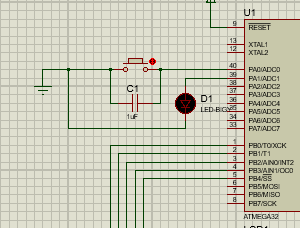
\includegraphics[width=0.7\textwidth]{solution/images/schematics2.png}
}

%----------------------------------------------------------------------------------------
%	SIMULATION SUBSECTION
%----------------------------------------------------------------------------------------

\subsection{Simulation}
\subsubsection{When button is not pressed}
The led is not emitting light and LCD outputs Off. \\\\

\centerline{
	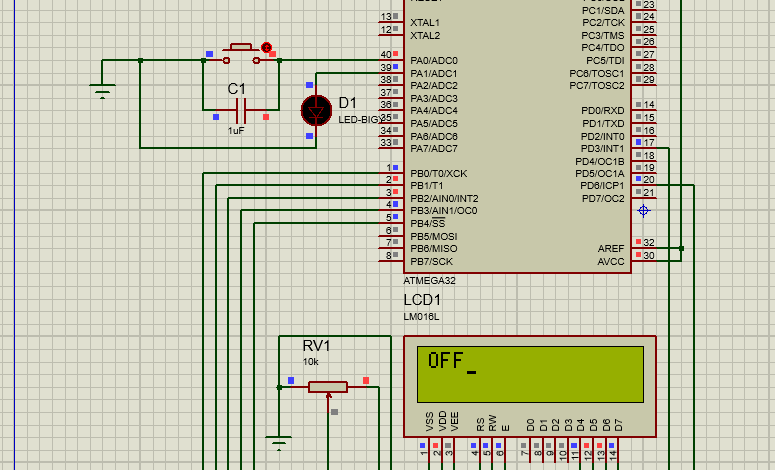
\includegraphics[width=0.6\textwidth]{solution/images/result1.png}
}

\subsubsection{When button is not pressed}
The led is emitting light and LCD outputs On. \\\\

\centerline{
	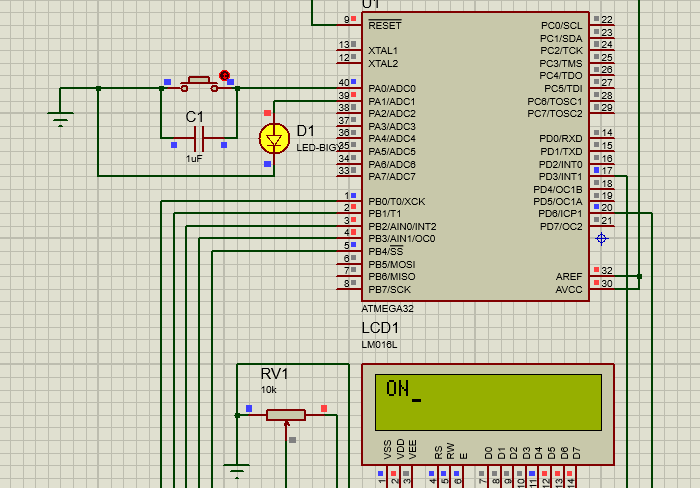
\includegraphics[width=0.6\textwidth]{solution/images/result2.png}
}

